Wir wollen nun eines der wichtigsten Werkzeuge f"ur die Analyse von diskreten \gls{lti}-Systemen einf"uhren und untersuchen.
Die $z$-Transformation nimmt f"ur diskrete \gls{lti}-Systeme dieselbe Rolle ein, wie die Laplace-Transformation f"ur zeitstetige \gls{lti}-Systeme.
Wir werden sehen, dass die Faltungs-Formel \eqref{eq:lti_sys:conv} im $z$-Bereich eine einfachere Form annimmt.
Au"serdem erlaubt uns die Transformation eine neue Sicht auf diskrete Systeme zu gewinnen, mit welcher es eventuell einfacher sein sollte gewisse Eigenschaften von Systemen nachzupr"ufen.
Wir werden auch sehen, dass sich manche Signale oder Systeme im $z$-Bereich kompakter aufschreiben lassen.

Die $z$-Transformation $X_\z: \C \rightarrow \C$ eines Signals $x[\cdot] : \N \rightarrow \C$ ist die komplexe Potenzreihe\footnote{\url{https://mathworld.wolfram.com/LaurentSeries.html}}
\begin{equation}\label{eq:ztrafo:def}
    z \mapsto X_\z(z) = \Sum{n\in\Z}{}{x[n] z^{-n}}.
\end{equation}
Wegen der Summation "uber ganz $\Z$ ist $X_\z(z)$ f"ur jedes $z$ ein Grenzwert, der nicht existieren muss.
Das hei"st, es ist notwendig auch \emph{immer} den Konvergenzbereich, oder Englisch die \gls{roc}, von $X_\z$ anzugeben.

Betrachten wir beispielsweise \[x[\cdot] = \{5,6,\Start{3},4,-\pi\},\] dann ergibt sich \[X_\z(z) = 5 z^2 + 6 z + 3 + 4z^{-1} - \pi z^2 \Text{mit \gls{roc}} \C \setminus \{0\}.\] 
Im Fall von $x[\cdot] = \delta[\cdot-k]$, ergibt sich $X_\z(z) = z^{-k}$ mit \gls{roc} $\C \setminus \{0\}$, wobei sich bei $x[\cdot] = \delta[\cdot+k]$, sich $X_\z(z) = z^{k}$ mit \gls{roc} $\C$ ergibt.
Man sieht nun auch, weshalb das System, das ein Signal um einen Abtastwert verz"ogert, oft mit $z^{-1}$ bezeichnet wird, weil dies die $z$-Transformation dessen Impulsantwort ist.
Au"serdem kann man bei endlichen Signalen im $z$-Bereich deren Werte im Zeitbereich einfach ablesen. 
Will man den Wert $x[n]$, also an Sample $n$, ermittelt man diesen, indem man den Koeffizienten vom passenden $z^{-n}$ betrachtet. 

Aber auch f"ur unendlich lange Signale, wie beispielsweise $x[n] = a^n u[n]$, ergibt sich
\[
X_\z(z) 
    = 1 + a z^{-1} + a^2 z^{-2} + \dots
    = \Sum{n = 0}{\infty}{
        a^n z^{-n}
    }
    = \Sum{n = 0}{\infty}{
        \left(a z^{-1}\right)^n
    },
\]
was eine geometrische Reihe "uber $az^{-1}$ darstellt. 
Dann folgt, dass
\[
    X_\z(z) = \frac{1}{1 - a z^{-1}},
\]
wobei diese Potenzreihe nur konvergiert, wenn $z > a$.
Das hei"st, dass die \gls{roc} hier alle $z \in \C$ umfasst mit $\Abs{z} > a$.
Wir sehen, dass sich eigentlich unendlich lange Signale im $z$-Bereich durch Berechnen des Grenzwertes knapper darstellen lassen.
Gleichzeitig k"onnen wir so auch die \gls{roc} bestimmen, indem wir ermitteln, wann der ermittelte Grenzwert existiert.

Wenn wir $z = r\exp(\jmath \phi)$ in die Definition \eqref{eq:ztrafo:def} einsetzen und $\Abs{X_\z(z)}$ betrachten, finden wir
\[
\Abs{X_\z(z)} 
    = \Abs{\Sum{n\in\Z}{}{x[n] z^{-n}}}
    \leqslant \Sum{n\in\Z}{}{\Abs{x[n] z^{-n}}}
    = \Sum{n\in\Z}{}{\Abs{x[n] r^{-n}} \Abs{\exp(- \jmath n \phi)}}
    = \Sum{n\in\Z}{}{\Abs{x[n] r^{-n}}}.
\]
Betrachten wir den letzten Ausdruck genauer indem wir ihn in zwei Summationen aufteilen, also
\[
\Sum{n\in\Z}{}{\Abs{x[n] r^{-n}}} 
    = \Sum{n=-1}{-\infty}{\Abs{x[n] r^{-n}}}
    + \Sum{n=0}{+\infty}{\Abs{x[n] r^{-n}}}
    = \Sum{n=1}{+\infty}{\Abs{x[-n] r^{n}}}
    + \Sum{n=0}{+\infty}{\Abs{\frac{x[n]}{r^{n}}}}.
\]
Das ergibt dann also, dass
\[
    \Abs{X_\z(z)} 
        \leqslant \Sum{n=1}{+\infty}{\Abs{x[-n] r^{n}}}
        + \Sum{n=0}{+\infty}{\Abs{\frac{x[n]}{r^{n}}}}
\]
Damit $X_\z$ existiert, m"ussen beide Grenzwerte existieren.
Der erste Grenzwert existiert, wenn es ein $r_1$ gibt, sodass $r_1^n$ die Werte $x[-n]$ so gewichtet, das sich Konvergenz einstellt. 
Dieses $r_1$ ist ausschlie"slich durch die Werte in der \q{Vergangenheit} von $x[\cdot]$ bestimmt! 
Wenn sich Konvergenz f"ur ein $r_1$ einstellt, dann auch f"ur alle $r < r_1$.
Der Konvergenzbereich ergibt sich also als ein Kreis mit Radius $r_1$.
Der zweite Grenzwert existiert, falls f"ur ein $r_2 > 0$ die Werte $1/r_2^n$ so die \q{Zukunft} von $x[n]$ so wichten, dass die Summe konvergiert.
Das hei"st, falls so ein $r_2$ existiert, dann konvergiert der zweite Summand f"ur alle $r > r_2$.

Die \gls{roc} ist also die Schnittmenge von der Menge $\{\Abs{z} \leqslant r_1\}$ mit der Menge $\{\Abs{z} \geqslant r_2\}$.
Dies ist in \Cref{fig:ztrafo:roc} zusammengefasst. Wir sehen auch, dass im Falle von $r_1 > r_2$ die \gls{roc} die leere Menge ist und deshalb die $z$-Transformation nicht existiert.

\begin{figure}
    \centering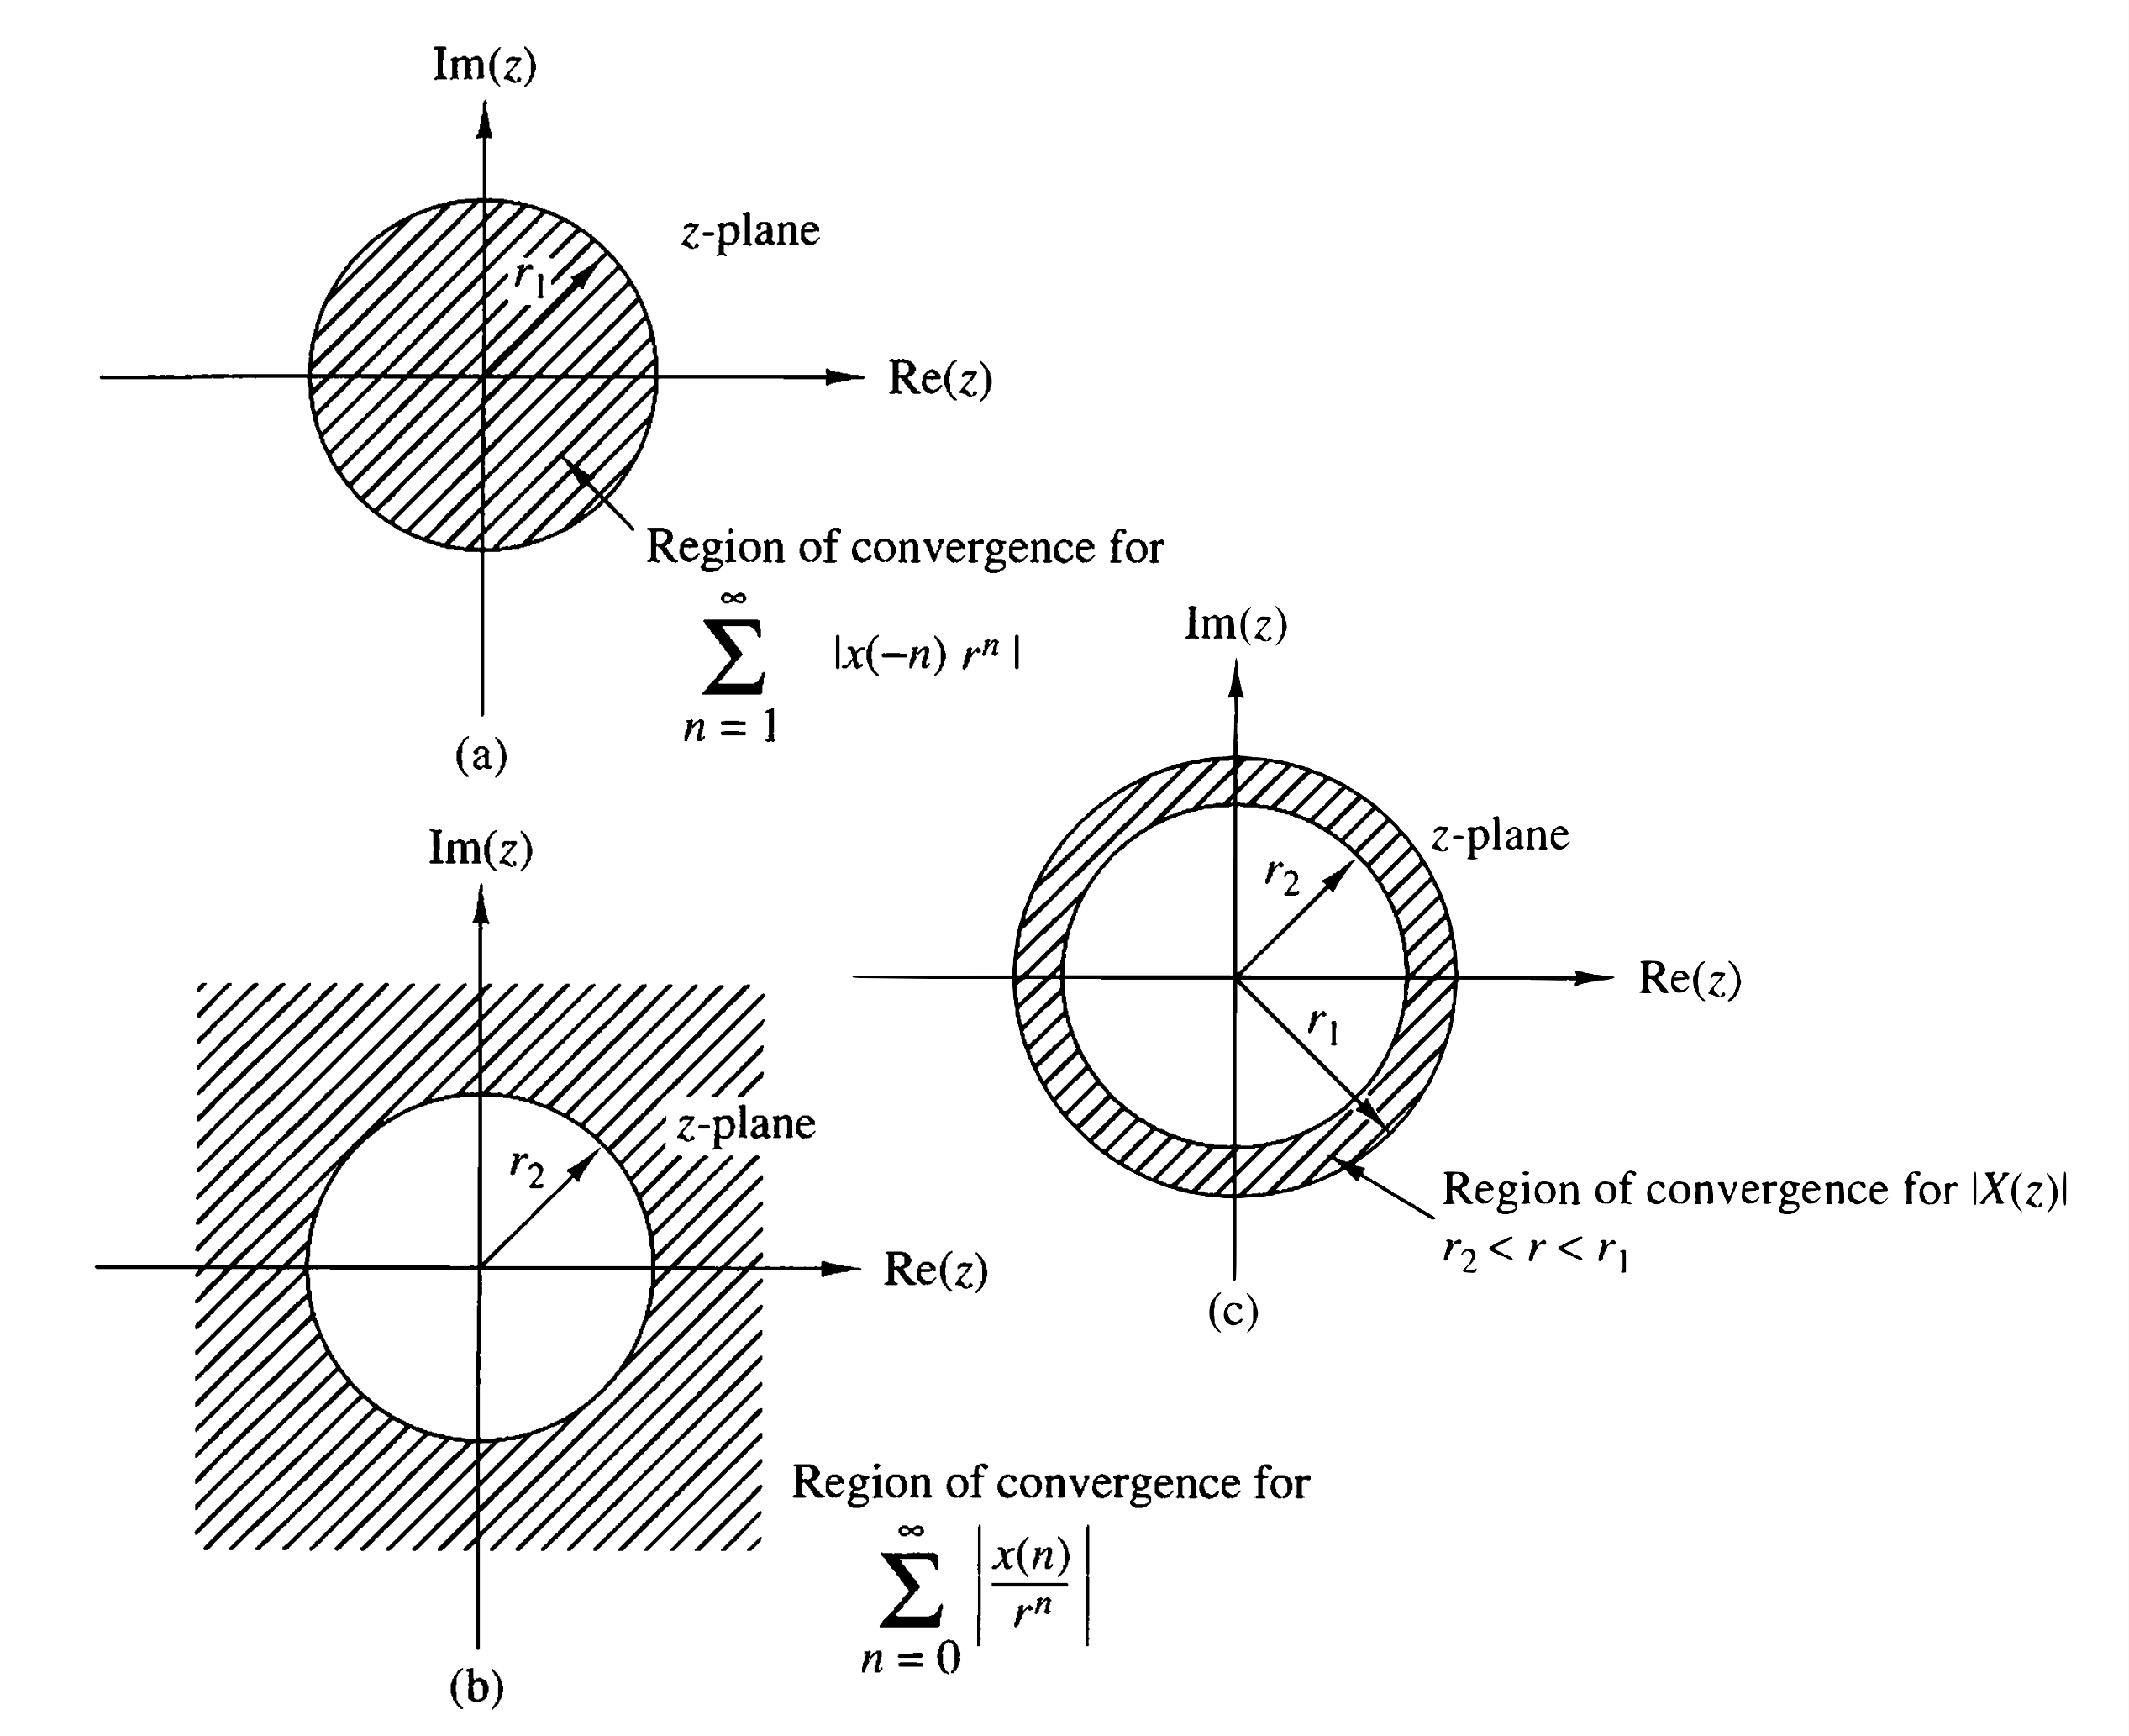
\includegraphics[width=0.8\textwidth]{img/ztrafo/roc.png}
    \caption{Veranschaulichung der Entstehung der \gls{roc} aus den Konvergenzkriterien. Quelle: \cite{proakis2013}}\label{fig:ztrafo:roc}
\end{figure}
\begin{itemize}
    \item eigenschaften: linear, timeshift (intuition mit koeffizienten), zeitumkehrung(intuition mit spiegelung am einheitskreis), ableitung in $z$-Bereich (analogie zu fourier)
    \item faltungseigenschaft
    \item algo: beide sequenzen $z$-trafo, multiplikation, inverse $z$-trafo
    \item inverse: tabelle \cite[tabelle 3.3]{proakis2013}, allgemeine invertierung: schwierig
    \item alle eigenschaften: \cite[tabelle 3.2]{proakis2013}
    \item anwendung: korrelation von signalen
    \item uebung: problem 3.6 in \cite{proakis2013}, initial value theorem, some plots aus \cite{proakis2013}
    \item rationale z-trafos: definition, pole-nullstellen, umkehrung: von pole-nullstellen zu $X(z)$
    \item ausfuehrliche diskussion von \cite[fig 3.3.5, 3.3.6]{proakis2013} 
    
\end{itemize}

\subsection{Kreuz- und Autokorrelation}\label{corr}

\begin{itemize}
    \item Anwendung $z$-Trafo: M-Sequenzen? polynome analysieren, wann maximale laenge?
    \item Definition
    \item eigenschaften
    \item synthetisches beispiel schwingung + noise, akf zeigt periodizitaet
    \item beispiel mit woelfer sunspot numbers
    \item beispiel mit m-sequenzen, niklas einladen, schaltung zeigen
    \item monster uebung: 2.65
\end{itemize}
